\documentclass[journal]{IEEEtran}
\usepackage[numbers]{natbib}
\usepackage{pgfplots}
\pgfplotsset{compat=1.18}
\usepackage{amsmath,amsfonts}
\usepackage{algorithmic}
\usepackage{array}
\usepackage{subcaption}
\usepackage{textcomp}
\usepackage{stfloats}
\usepackage{verbatim}
\usepackage{booktabs}
\usepackage{multirow}
\usepackage{graphicx}
\usepackage{colortbl}
% \usepackage[table,xcdraw]{xcolor}
\usepackage{tikz}
\usepackage{titlesec}
\usepackage{authblk}
\usepackage{marvosym}
\usetikzlibrary{positioning, calc}
\usetikzlibrary{arrows}
\newcolumntype{P}[1]{>{\raggedright\arraybackslash}p{#1}}

\hyphenation{op-tical net-works semi-conduc-tor IEEE-Xplore}
% \def\BibTeX{{\rm B\kern-.05em{\sc i\kern-.025em b}\kern-.08em
    % T\kern-.1667em\lower.7ex\hbox{E}\kern-.125emX}}
% \usepackage{balance}
\begin{document}
\title{bnmetamodel 2.0}

\author[1]{T. Griffiths\thanks{\textsuperscript{\Cross}Corresponding author: t.griffiths20@imperial.ac.uk}}
\author[2]{Z. Xuereb Conti}
\author[1]{M. Bluck}

\affil[1]{Department of Mechanical Engineering, Imperial College London, UK}
\affil[2]{Data-Centric Engineering / TRIC:DT, The Alan Turing Institute, UK}
\vspace{-15pt}

\maketitle

\begin{abstract}

\end{abstract}

\begin{IEEEkeywords}
Fusion power, metamodels, surrogate modelling, fusion commercialisation, machine learning, fusion economics, energy, Bayesian Networks
\end{IEEEkeywords}
\vspace{-2ex}

\section{Introduction}

Commercial-scale fusion power holds the promise of delivering reliable baseload electricity, reducing carbon emissions, and enhancing energy security. However, techno-economic modeling of future fusion power plants faces challenges due to uncertain and imprecise costing models. To address this uncertainty, probabilistic methods have been demonstrated to estimate fusion power economics effectively~\cite{Griffiths2024}

Despite the challenges, it's vital for the fusion community to persist in researching both technical and economic performance metrics. The advancement of nuclear fusion research is propelled by a multitude of scientific pursuits in modeling and analysis, drawing upon expertise in theory, experimentation, computation, and inference. Fusion reactions involve intricate processes at extreme conditions within the reactor. Deterministic, theoretical and numerical models must accurately capture these extreme conditions through plasma dynamics, energy transfer, and reaction kinetics. Yet, they often struggle to handle uncertainties inherent in plasma behavior fluctuations and in external factors such as magnetic field perturbations. These uncertainties can significantly impact predicted reactor performance, making consistent achievement of desired output parameters challenging, thus hindering reactor design in roadmapping and slowing R\&D. While significant advancements have been made in fusion research, our understanding of plasma physics, fusion reactions, and reactor engineering continues to evolve. Deterministic models may lack the adaptability to incorporate emerging insights or experimental data, potentially leading to discrepancies between predicted and observed reactor behavior. Failing to address these challenges could hinder investment attraction, roadmap target achievement, and the promotion of additional investment opportunities. Implementing statistical methods, like sensitivity analyses, can help assess key modeling variables, identify areas for improvement, and enhance prediction reliability.

Machine Learning (ML) models offer a valuable tool for developing understanding in areas lacking experimental data. They provide the flexibility to simulate various scenarios and conditions rapidly, enabling quick iteration and parameter modification. This facilitates swift exploration and optimisation of designs without the need for physical modifications or repeated experiments. Given the complexity of fusion engineering systems, ML models can effectively handle numerous variables and interactions, facilitating the analysis of large-scale systems with intricate behaviours.

This study extends the surrogate modelling technique applied in~\cite{Griffiths2024} to a new case study, introducing enhancements and modifications to the methodology. The objective is to expand the application of Bayesian Networks (BNs) for a deeper understanding of fusion power design spaces. It introduces an innovative, probabilistic approach to managing uncertainty in fusion research, diverging from traditional techniques. The objective of surrogate modelling is to develop a streamlined representation that mirrors the outcomes of a complex deterministic numerical or theoretical model, accounting for its various inputs and parameters. In this scenario, a BN serves as a proxy for a fusion systems code enabling the replication of a spheerical tokamak in its design phase, forecasting the economic and performance viability amidst data uncertainties.

The use of probabilistic Bayesian inference with a Bayesian Network in this analysis offers several advantages over other surrogate modeling techniques. Unlike deterministic models, Bayesian inference accounts for uncertainties in input parameters and output responses, providing a probabilistic framework that captures the inherent variability in fusion systems. Furthermore, Bayesian inference facilitates the integration of prior knowledge and observational data, enabling more robust inference and decision-making in complex engineering systems like fusion reactors. Overall, leveraging Bayesian inference allows fusion developers to extract actionable insights from limited experimental data and make informed design decisions that maximise the performance and cost-effectiveness of fusion reactor systems.

The present investigation expands upon the surrogate modeling framework initially proposed by Griffiths et al.~\cite{Griffiths2024} through several notable enhancements. Firstly, it introduces an enhanced and refined methodology, detailed in Section~\ref{sec:methodology}, to address limitations identified in the previous work. Secondly, it incorporates steps for validation and examines the influence of hyperparameters on the proof-of-concept BN, a feature lacking in~\cite{Griffiths2024} due to constraints on publication word count. Thirdly, the study shifts its focus to applying the improved methodology to a new case study, leveraging data from a private fusion developer to explore uncertain parameters of fusion power plants. A notable enhancement is the inclusion of multiple output nodes, distinguishing this study and strengthening the model's capability to address various outputs crucial to developers. Unlike in~\cite{Griffiths2024}, the input and output data in this study represent a fusion reactor still in its design phase, offering a more practical example of how the BN can support ongoing engineering decisions, enabling real-time optimisation and feedback for fusion developers.

The paper's structure is as follows: Section~\ref{sec:BNs} provides an overview of BNs and their suitability in aid in fusion research in the methodological framework of surrogate modelling. Section~\ref{sec:background} provides a comprehensive literature review, Section~\ref{sec:methodology} outlines the refined methodology with illustrative examples from the proof-of-concept presented in~\cite{Griffiths2024}, Section~\ref{sec:res_decision} details the implementation of the BN in a new case study, Section~\ref{sec:Discussion} discusses the implications of the BN's results on the fusion developer's design approach, and Section~\ref{sec:conc} concludes the paper, along with suggestions for future research directions.

\section{Bayesian Networks}\label{sec:BNs}

\begin{figure}[t]
    \centering
    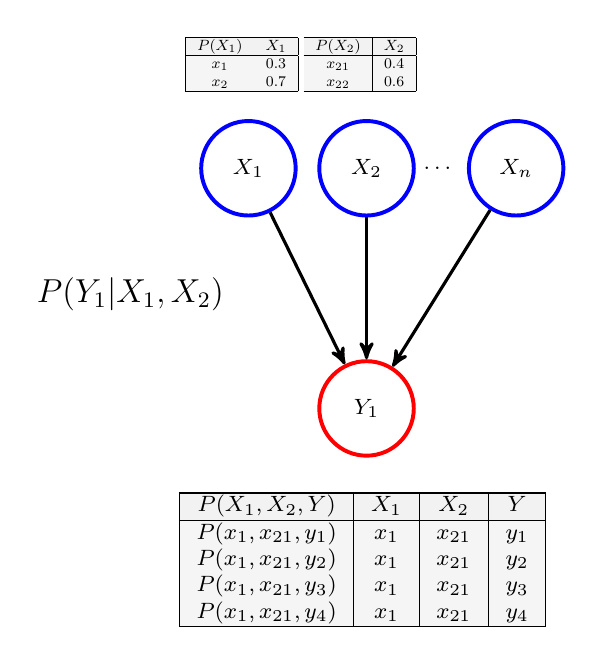
\begin{tikzpicture}[node distance=1.5cm, font=\footnotesize, align=center, >=stealth', line width=0.5mm]
        % Define colors
        \definecolor{lightgreen}{rgb}{0.56, 0.93, 0.56}
        \definecolor{lightred}{rgb}{0.98, 0.5, 0.45}

        % Nodes
        \node[draw, circle, draw=blue, text=black, minimum size=1.2cm] (input1) {$X_1$};
        \node[draw, circle, draw=blue, text=black, right of=input1, minimum size=1.2cm] (input2) {$X_2$};
        \node[right of=input2, node distance=0.9cm] (dots) {$\ldots$};
        \node[draw, circle, draw=blue, text=black, right of=dots, node distance=1cm, minimum size=1.2cm] (inputn) {$X_n$};
        % Probability expression
        \node[left of=input1, node distance=1.5cm, yshift=-1.6cm, font=\large] (prob) {$P(Y_1 | X_1, X_2)$};

        \node[draw, circle, draw=red, text=black, below=1.8cm of input2, minimum size=1.2cm] (output1) {$Y_1$};

        % Edges
        \foreach \i in {1,2,n} {
            \draw[->, line width=0.4mm] (input\i) -- (output1);  % Decreased line width
        }
        \node[above=0.2cm of input1] {
            \resizebox{1.5cm}{!}{%  <-- set the width of the table here
                \begin{tabular}{|c|c|}
                    \hline
                    \rowcolor{gray!10}
                    $P(X_1)$ & $X_1$ \\
                    \hline
                    \rowcolor{gray!8}
                    $x_1$ & 0.3 \\
                    \rowcolor{gray!8}
                    $x_2$ & 0.7 \\
                    \hline
                \end{tabular}
            }
        };

        \node[above=0.2cm of input2] {
            \resizebox{1.5cm}{!}{%  <-- set the width of the table here
                \begin{tabular}{|c|c|}
                    \hline
                    \rowcolor{gray!10}
                    $P(X_2)$ & $X_2$ \\
                    \hline
                    \rowcolor{gray!8}
                    $x_{21}$ & 0.4 \\
                    \rowcolor{gray!8}
                    $x_{22}$ & 0.6 \\
                    \hline
                \end{tabular}
            }
        };
        \node[below=0.3cm of output1] {
            %\resizebox{1.5cm}{!}{
                \begin{tabular}{|c|c|c|c|}
                    \hline
                    \rowcolor{gray!10}
                    $P(X_1, X_2, Y)$ & $X_1$ & $X_2$ & $Y$ \\
                    \hline
                    \rowcolor{gray!8}
                    $P(x_1, x_{21}, y_1)$ & $x_1$ & $x_{21}$ & $y_1$ \\
                    \rowcolor{gray!8}
                    $P(x_1, x_{21}, y_2)$ & $x_1$ & $x_{21}$ & $y_2$ \\
                    \rowcolor{gray!8}
                    $P(x_1, x_{21}, y_3)$ & $x_1$ & $x_{21}$ & $y_3$ \\
                    \rowcolor{gray!8}
                    $P(x_1, x_{21}, y_4)$ & $x_1$ & $x_{21}$ & $y_4$ \\
                    \hline
                    % Rest of the JPD table entries...
                    % ...
                \end{tabular}
            %}
        };        
       
    \end{tikzpicture}
    \caption{\small Graphical representation of BN where nodes $X_i$ represent the input variables and the node $Y_1$ represents the output variable to the analytical model. The solid lines represent the existing nodes in the model. The double-edged arrow represents additional information.}\label{fig:BN3} 
    %\vspace{-15pt}
\end{figure}

Under the umbrella of ML lies a multitude of computational algorithms, each with their own unique characteristics. Despite their diversity, they all share the fundamental trait that they are not programmed to solve specific tasks. Instead, they undergo iterative learning, gradually refining their performance through experience gained from previous iterations. Whilst learning, an ML algorithm utilises a statistical model with adjustable parameters that minimises a loss function through adjustment of internal parameters. For instance, in regression tasks, where the algorithm aims to align its output with a target value, common metrics like mean square error are often employed to evaluate its performance. The training process can be likened to a fitting routine, wherein the model, typically a highly flexible one such as a deep neural network (DNN), learns to capture intricate patterns within the data. The primary objective of training ML algorithms is to enable accurate predictions for new input data, requiring the them to learn solutions applicable beyond the training dataset. Generalisation, the ability to perform well on unseen data, serves as the primary criterion for evaluating an ML model's effectiveness. The main challenge lies in avoiding overfitting and enhancing generalisation. This challenge has led to the recent surge in popularity of deep learning (DL), which excels at approximating complex functions for high-dimensional input and output data, thereby offering solutions to real-world complex problems.

Within the realm of ML, Bayesian Networks (BNs) represent a notable approach, serving as a type of probabilistic graphical model that encapsulates a set of variables and their conditional dependencies through a directed acyclic graph (DAG)~\cite{Hand2001}. As ML algorithms aim to learn generalized solutions applicable beyond the training dataset, BNs offer a structured framework for capturing and representing probabilistic dependencies among variables. Unlike traditional ML approaches, BNs provide a more explicit representation of probabilistic relationships between variables, facilitating a deeper understanding of the underlying data generating process. This transition from ML to BNs underscores the shift from optimising predictive performance to gaining insight into the underlying mechanisms governing the data. Consequently, understanding BNs becomes increasingly valuable in leveraging the full potential of ML algorithms for real-world applications.

A BN consists of nodes representing variables and edges representing dependencies between variables. The parameters of a BN specify the conditional probabilities associated with each node given its parents in the network. These conditional probabilities determine the relationships and dependencies between variables in the BN.\@ When multiple probability distributions are combined, a Joint Probability Distribution (JPD) is formed.  The structure of the BN captures the dependencies between variables, and the conditional probabilities are derived from data or expert knowledge. It is not necessary to explicitly specify all the parameters of the JPD. This allows for efficient representation of the JPD without explicitly specifying all the individual parameters, making BNs a powerful tool for probabilistic modelling. This provides a compact representation by combining the \textit{local} conditional distributions for each node, with respect to its connected parent nodes~\cite{Koller2009}, see Figure~\ref{fig:BN3}. The joint probability distribution can be factorised into a product of conditional probability distributions, one for each variable given its parents in the graph. This factorisation is known as the chain rule of probability. Also known as the general product rule, this allows the calculation of any member of the joint distribution of a set of random variables using only conditional probabilities.

Given a set of random variables, say $X_1, X_2, \ldots, X_n$, the chain rule of probability states that the joint probability of these variables is the product of the conditional probabilities of each variable given all the variables that precede it. Mathematically, this can be expressed as:

\begin{align}
    P(X_1, X_2, \ldots, X_n) = & P(X_1) \nonumber \\
    & * P(X_2 | X_1) \nonumber \\
    & * P(X_3 | X_1, X_2) \nonumber \\
    & * \ldots \nonumber \\
    & * P(X_n | X_1, X_2, \ldots, X_n-1)
    \label{eq:chain_rule}
\end{align}
    
In Equation~\ref{eq:chain_rule}: $P(X1, X2, \ldots, Xn)$ is the joint probability of $X1$ through $Xn$. $P(X_i | X1, \ldots, X_i-1)$ is the conditional probability of $X_i$ given all the preceding variables.



\begin{figure*}[t]
    \centering
    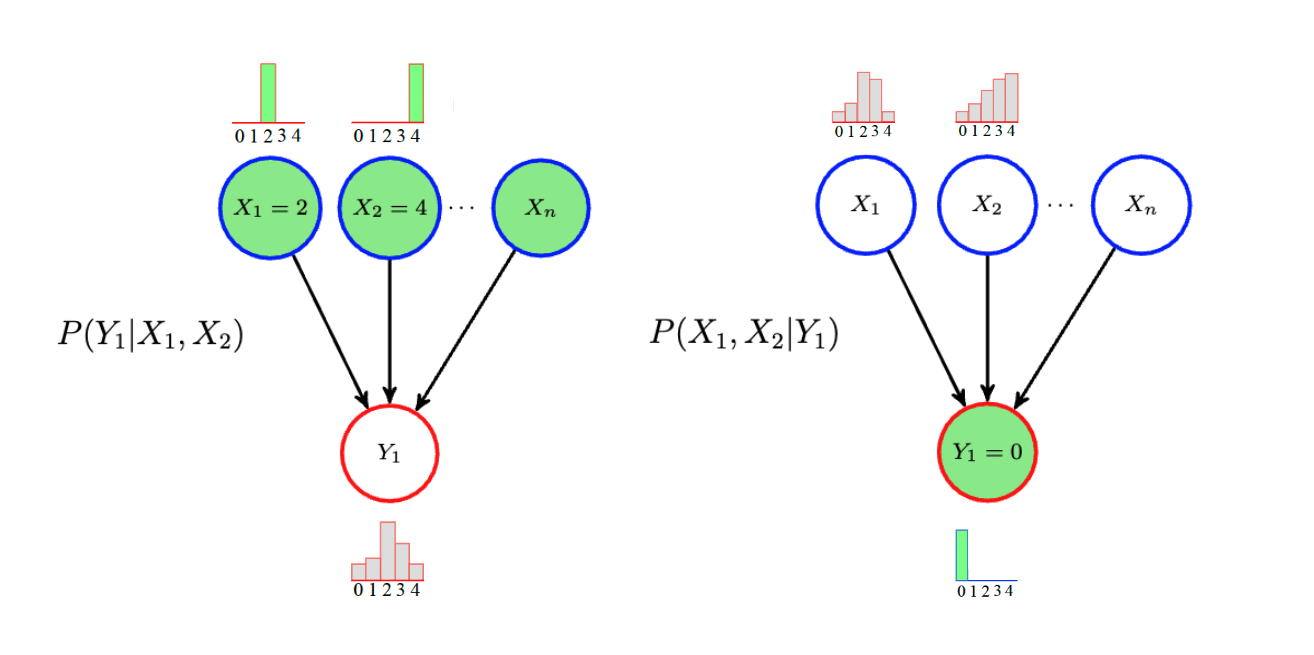
\includegraphics[width=0.75\textwidth]{figures/methodology/inference_F&R_diagram.png}
    \caption{A visual representation of Bayesian inference in the forward (left) and reverse (right) directions.}~\label{fig:inference_F&R_diagram}
\end{figure*}

In depth, the term \textit{prior} refers to the initial probability distribution assigned to a variable. On the other hand, the \textit{posterior} probability refers to the updated probability distribution after \textit{prior} beliefs are updated via \textit{inference}, based on available evidence. The primary benefit of a probabilistic representation lies in its ability to perform \textit{probabilistic inference}, which enables bi-directional reasoning with uncertain information using probabilistic methods. Thus, adopting a BN as a surrogate model facilitates exploration of causal relationships between fusion parameters and cost in both forward and reverse directions, allowing for an uncertain fusion parameter design space to be mapped from a desired target output range. 

By defining inference as the process of making deductions based on evidence, reasoning and, prior knowledge, it is possible to further characterise Bayesian inference as the act of making alterations to existing probability distributions to discover how, based on their causal relationships, the variable's remaining probability distributions are altered. This acts as a useful tool to measure and understand relationships between inputs and responses in engineering design spaces~\cite{Koller2009}. 

The interpretation of simulation outputs from analytical models can be challenging for leadin fusion developers without a deep understanding of the associated engineering or physics principles. This can result in reliance on uncertain numerical data, without the ability to leverage the causal structure of the numerical output. In this scenario, a BN can serve as a two-way translation medium between the overall fusion research and the engineering domains. The use of bi-directional inference can assist engineers in providing feedback in the form of design parameters, based on the interconnections between the two domains. In this manner, fusion researchers can impose constraints on the output distributions of the BN, leveraging their expertise and experience, while engineers and physicists handle the input distributions to interpret engineering constraints in terms of design parameters. The `translation' process facilitated by a BN could lead to more comprehensive decisions, as probabilistic inference considers the entire network of relationships between inputs and outputs during computation. This is in contrast to traditional deterministic models, which only consider the direct relationship between inputs and outputs. 

The ability to perform bi-directional inference is a key feature of BNs, as it allows for the prediction of outputs based on input data, \textit{forward inference}, and inputs based on output data, \textit{reverse inference}. This capability is particularly useful in the context of engineering design, as it enables the exploration of causal relationships between inputs and outputs, and the prediction of inputs based on desired outputs. This can provide valuable insights for decision-making and design optimisation, as it allows for the identification of input values that are most likely to result in a desired output, and the prediction of the likely output given a set of input values. Refer to Figure~\ref{fig:inference_F&R_diagram} for a visual representation of Bayesian inferene in the forward (left) and reverse (right) directions. 

In addition to its flexibility and robustness, probabilistic Bayesian inference can complement current methods in fusion research by providing a holistic understanding of reactor behaviour and performance. Different ways this technique can be used in conjunction with current methods to enhance fusion research include: integration with experimental data, uncertainty quantification, optimisation of experimental design, decision support for design iterations, and risk assessment and management.
    
\subsection{Literature review}~\label{sec:background}

At present, besides the antecedent proof-of-concept study, no known instances exist where BNs have specifically been employed as surrogates in fusion research~\cite{Griffiths2024}. Consequently, this section will delve into the application of ML in fusion research, with a particular focus on the utilisation of other Bayesian modeling techniques in surrogates and uncertainty quantification.

In a review article by Pavonne et al.\ a comprehensive overview of ML and Bayesian inference in fusion R\&D is provided~\cite{Pavone2023}. Bayesian inference facilitates the efficient utilization of shared information among heterogeneous experimental data sources concerning a common underlying description or model of a phenomenon. The study outlines fundamental Bayesian modeling for fusion experiments in physics models via inference of plasma equilibria~\cite{Svensson2003, Svensson2004}, Gaussian process (GP) tomography~\cite{Svensson2011}, and uncertainty propagation~\cite{Fischer2020, Fischer2010}. The application of ML in fusion research has encompassed various types, demonstrating the potential to address complex challenges in fusion reactor design and operation.

Pavone et al.~details significant studies employing trending ML techniques in fusion, particularly within the realm of deep learning (DL) methods in neural networks. Specifically, in the theory of artificial neural network (ANN) algorithms and convolutional neural networks (CNNs), the latter of which was utilised in~\cite{Pavone2019} for the Wendelstein 7-X Stellarator experiment to reconstruct ion and electron temperature profiles from 2D x-ray spectral images. The article underscores the significance of Bayesian inference for neural networks within the fusion community. Reinforcement learning (RL) has been employed in seminal studies for controlling tokamak plasmas~\cite{Degrave2022} and predicting disruptions~\cite{Kates2019}, showcasing applicability to practical tasks in real-time. In~\cite{Degrave2022}, RL enhanced flexibility in plasma control by generating non-linear feedback controllers, thereby simplifying the control system. The RL system learned the control policy through interaction with a simulated environment modeling the dynamic state of the plasma shape and current, magnetic diagnostics sensor data, coil currents, and controller dynamics. In~\cite{Kates2019}, a disruption mitigation system utilizing DL predicts potential disruptions, aiming to reduce thermal loads. The algorithm combines convolutional and recurrent neural networks (CNN and RNN, respectively), trained on data from the JET and DIII-D experiments. The CNN learns the temporal dynamics of the plasma and predicts the likelihood of disruptive states. If the system output exceeds a certain threshold, an alarm triggers the activation of a mitigation action. 


\begin{figure*}[t]
    \centering
    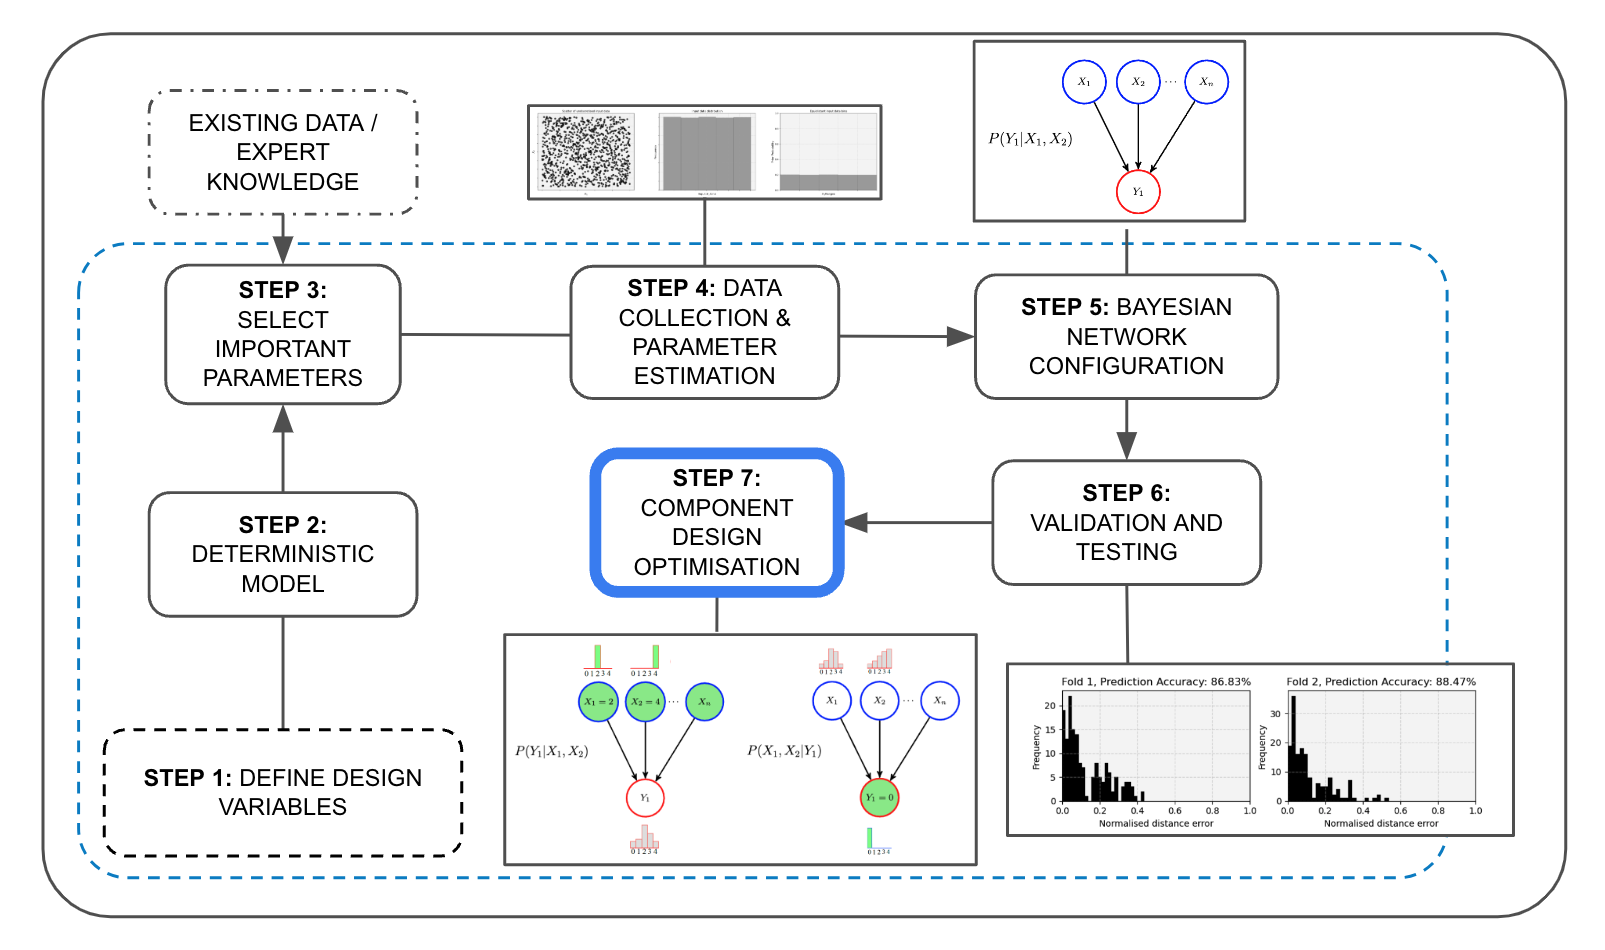
\includegraphics[width=0.9\textwidth]{figures/methodology/workflows/workflow_v5.png}
    \caption{Workflow of the surrogate modelling process, adapted from~\cite{Conti2019}, and refined from the methodology presented in~\cite{Griffiths2024}}~\label{fig:workflow}
\end{figure*}


Surrogate models aim to expedite computationally intensive models based on numerical approximations and theoretical first principles, a particularly crucial endeavor in fusion research, especially concerning turbulent transport computations. An illustrative case provided in~\cite{Van2020} demonstrates the efficacy of surrogate models: leveraging a dataset from~\cite{Citrin2017}, a neural network was trained. Integrated into modeling simulations, this neural network efficiently calculated the evolution of ion and electron temperature profiles as well as electron density profiles. The network delivered crucial values such as the main ion and electron heat flux and electron particle flux at a remarkable speed—864 times faster than a numerical model requiring four times the number of cores. Similar instances of neural networks serving as surrogates can be found in~\cite{Meneghini2017}, focusing on turbulent transport calculations, and~\cite{Miller2021}, exploring physics-informed plasma behavior in a particle-in-cell gyrokinetic code.

Pavone et al.\ also shed light on the computational complexity inherent in Bayesian inference, particularly in sampling from the posterior distribution. They elucidate that while Markov Chain Monte Carlo (MCMC) methods offer a means to sample from the posterior, their practicality diminishes in many real-world scenarios due to the substantial number of iterations required. The primary bottleneck arises from the need to compute the likelihood function, which entails running a forward modelz or simulation code—a process often prohibitively slow in complex systems. Pavone and colleagues argue that deep learning (DL) models offer a promising alternative, demonstrating their ability to efficiently reconstruct the posterior and infer plasma parameters from diagnostic data within short time frames, as evidenced in studies such as those by Pavone et al.~\cite{Pavone2018,Pavone2019, Pavone2020, Pavone2021}

In navigating the landscape of fusion research, the interplay between machine learning (ML) techniques and Bayesian inference emerges as a pivotal force, offering novel avenues for addressing complex challenges. While BNs have yet to find widespread application as surrogates in fusion studies, the realm of ML, bolstered by Bayesian modeling techniques, presents a rich tapestry of possibilities. From the nuanced inference of plasma equilibria to the predictive power of deep learning methods like convolutional neural networks (CNNs), researchers navigate a diverse array of methodologies to elucidate the intricacies of fusion phenomena. As surrogate models expedite computations and DL models offer efficient alternatives to Bayesian inference, the fusion community stands at the precipice of transformative discovery, guided by the symbiotic relationship between traditional methodologies and cutting-edge computational techniques.

\section{Methodology}\label{sec:methodology}

In this section, aa set of general procedures for creating and applying a BN as a surrogate model is presented, drawing inspiration from~\cite{Conti2019} and leveraging insights from the proof-of-concept study~\cite{Griffiths2024}. Illustrated in Figure~\ref{fig:workflow}, a stepwise algorithm delineates the creation, cross-validation, and application of the BN surrogate model, applicable to various input-output problems. This algorithm has been refined and optimised from previous methodologies. In this study, steps are explored methodologically, focusing on identifying optimal deployment strategies such as specific hyperparameters and validation techniques. Throughout the explanation of these steps, specific adaptations and enhancements are highlighted to the previous approach, illustrating how they were implemented in the proof-of-concept study.

\subsection{\textbf{Step 1}: Define design variables}\label{sec:design}

In this step, a strategic decision is made regarding the focal point of the model, whether it targets a whole reactor system or a critical component such as the breeder blanket or the divertor. Following this decision, the key parameters and characteristics of the chosen component are then identified and defined as input variables, labeled as $X_1$, $X_2$, \ldots, $X_n$. As exemplified in the proof-of-concept study conducted by Griffiths et al.~\cite{Griffiths2024}, this process involved the conceptualization of a future-type spherical tokamak reactor system to conduct a comprehensive investigation into its economic viability. In this study, the inputs and outputs of the model were framed as the design variables, allowing for a holistic evaluation of the power plant's economics.

Ahead of executing the selected analytical model, it requires configuration. This process includes choosing the inputs and outputs, along with defining the value ranges for each variable. The selection of inputs and outputs is guided by the objectives of the analysis and the data at hand. The value ranges for each variable are set considering the system's physical limitations and the required granularity of the analysis. Once configured, the analytical model is run to produce the dataset, which is then utilised to set up the BN.~Typically, BNs perform better at making predictions when the input distribution is uniform. This is for several reasons: model assumptions: normal distributions assume a bell-shaped curve with values concentrated around a mean, while uniform distributions make no assumptions about data shape and better capture the true underlying distribution. Nonlinearity and Outliers: normal distributions are sensitive to outliers, as they can significantly impact the mean and standard deviation, which may not accurately represent the underlying relationship between variables. Uniform distributions, being less influenced by extreme values, can provide a more robust representation of the data. Flexibility and Non-parametric Modelling: Uniform distributions offer flexibility in modelling unknown or non-normally distributed data without relying on specific distribution assumptions, allowing the BN to adapt and capture complex relationships. Simplification of model complexity: normal distributions require additional parameters (mean and standard deviation) that necessitate estimation, increasing model complexity and the number of parameters to learn. In contrast, using uniform distributions simplifies the model by eliminating the need for extra parameter estimation, resulting in easier training and interpretation~\cite{Duda1973,Neapolitan2004, Koller2009}.

\begin{figure*}[t]
    \centering
    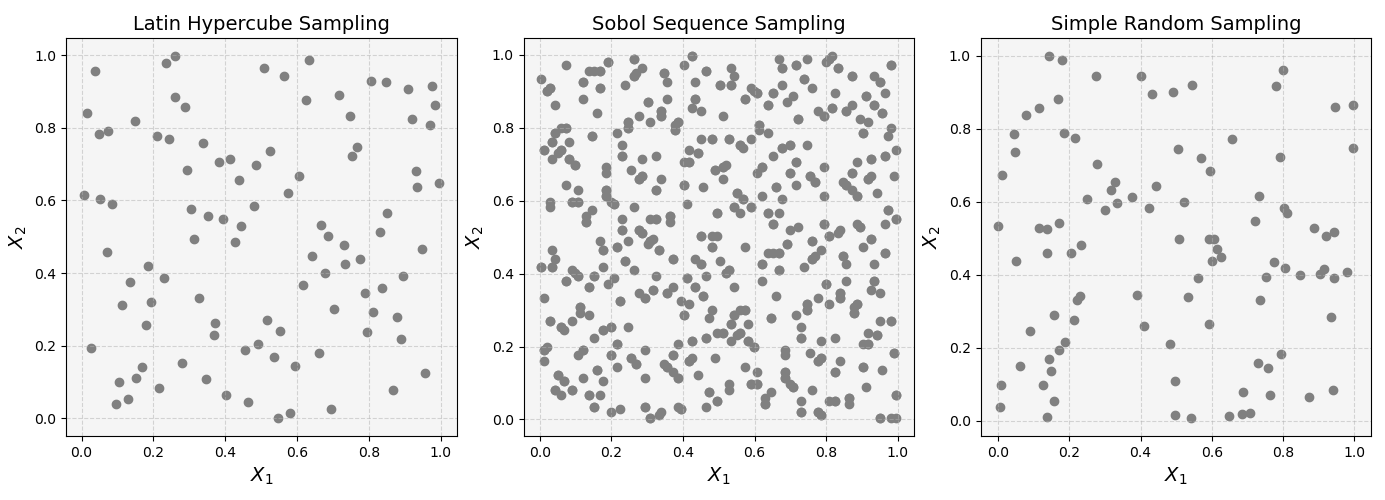
\includegraphics[width=0.8\textwidth]{figures/methodology/sobol_vs_lhs_simple.png}
    \caption{\small A comparison of the Sobol and Latin Hypercube sampling methods.}~\label{fig:sobol_vs_lhs}
\end{figure*}

\subsection{\textbf{Step 2}: Deterministic model}\label{sec:deterministic}
The deterministic model serves as a foundation for the BN, incorporating a range of models rather than being restricted to a single one. Its primary function is to generate output variables, denoted as $Y_1$, $Y_2$, \ldots, $Y_m$, which serve as the foundation for data collection and parameter estimation in developing the surrogate model. Drawing from the proof-of-concept study by Griffiths et al.~\cite{Griffiths2024}, an illustrative example of this step involves the utilization of the UKAEA systems code, PROCESS~\cite{Kovari2014, Kovari2016}. This model examines the interconnection between the engineering and physics subsystems comprising a fusion power plant while accommodating user-defined constraints.

\subsection{\textbf{Step 3}: Parameter Selection}\label{sec:parameters} 
In this stage, the focus is on identifying and selecting input parameters that wield substantial influence over the output variables modeled by the deterministic model. This task demands careful deliberation and expertise to discern the most pertinent parameters governing the system's behavior and performance.

In the study by Griffiths et al.~\cite{Griffiths2024}, an example illustrates this process. They utilised an ST design basis from a previous work by the same authors, presenting a comprehensive techno-economic analysis of ST fusion power plants for hybrid hydrogen-electricity production~\cite{Hidalgo-Salaverri2023}. To lay the groundwork for the techno-economic investigation, which encompassed evaluations under optimistic, moderate, and conservative scenarios, a rigorous sensitivity analysis was conducted. The objective was to streamline the problem's complexity by screening other potentially economically significant parameters.

Inputs were delineated as the reactor's design parameters, including the Greenwald fraction W impurity fraction Current drive efficiency factor Aspect ratio Toroidal field on axis [T]
Total plasma beta NBI plug efficiency Turbine inlet temperature [ºC]. Outputs, on the other hand, were characterized as the economic parameters of the reactor, such as the capital cost [millions USD\$]. The ranges for each variable were established considering the system's physical constraints, the required level of analysis granularity, and existing values derived from ST design bases documented in the literature.

\subsection{\textbf{Step 4}: Data Collection and Parameter Estimation}\label{sec:data} 


Here, the deterministic model is executed to gather data required to configure the surrogate model. It's imperative to collect comprehensive data representing the entire design space to ensure the surrogate model's accuracy. Specific sampling techniques such as Latin Hypercube or Sobol sampling are employed to ensure the collected data adequately covers the design space. Figure~\ref{fig:sobol_vs_lhs} illustrates the sampling of the input space. The collected data is then utilized to configure the surrogate model. 

For example, the final phase of~\cite{Hidalgo-Salaverri2023} focused on employing a Sobol analysis, which generated the dataset for~\cite{Griffiths2024}. The input space was sampled between the parameter limits using Saltelli's extension of the Sobol sequence~\cite{Sobol2001, Saltelli2002}; a quasi-random low-discrepancy sequence used to generate uniform samples of parameter space~\cite{Herman2023}. This analysis extensively investigated the influence of input parameters on the variance of the output, capital cost, by executing PROCESS $>$10,000 times. The analysis considered first-order ($S_{1}$), second-order ($S_{2}$), and complete interaction effects ($S_{\text{tot}}$), thus identifying key economic parameters and their interrelationships, conceptualising the design space of the nodes for the BN.\@

\subsection{\textbf{Step 5}: Bayesian Network Configuration}\label{sec:BNconfiguration}

\begin{figure*}[t]
    \centering
    \begin{minipage}{\textwidth}
        \begin{subfigure}{\textwidth}
            \centering
            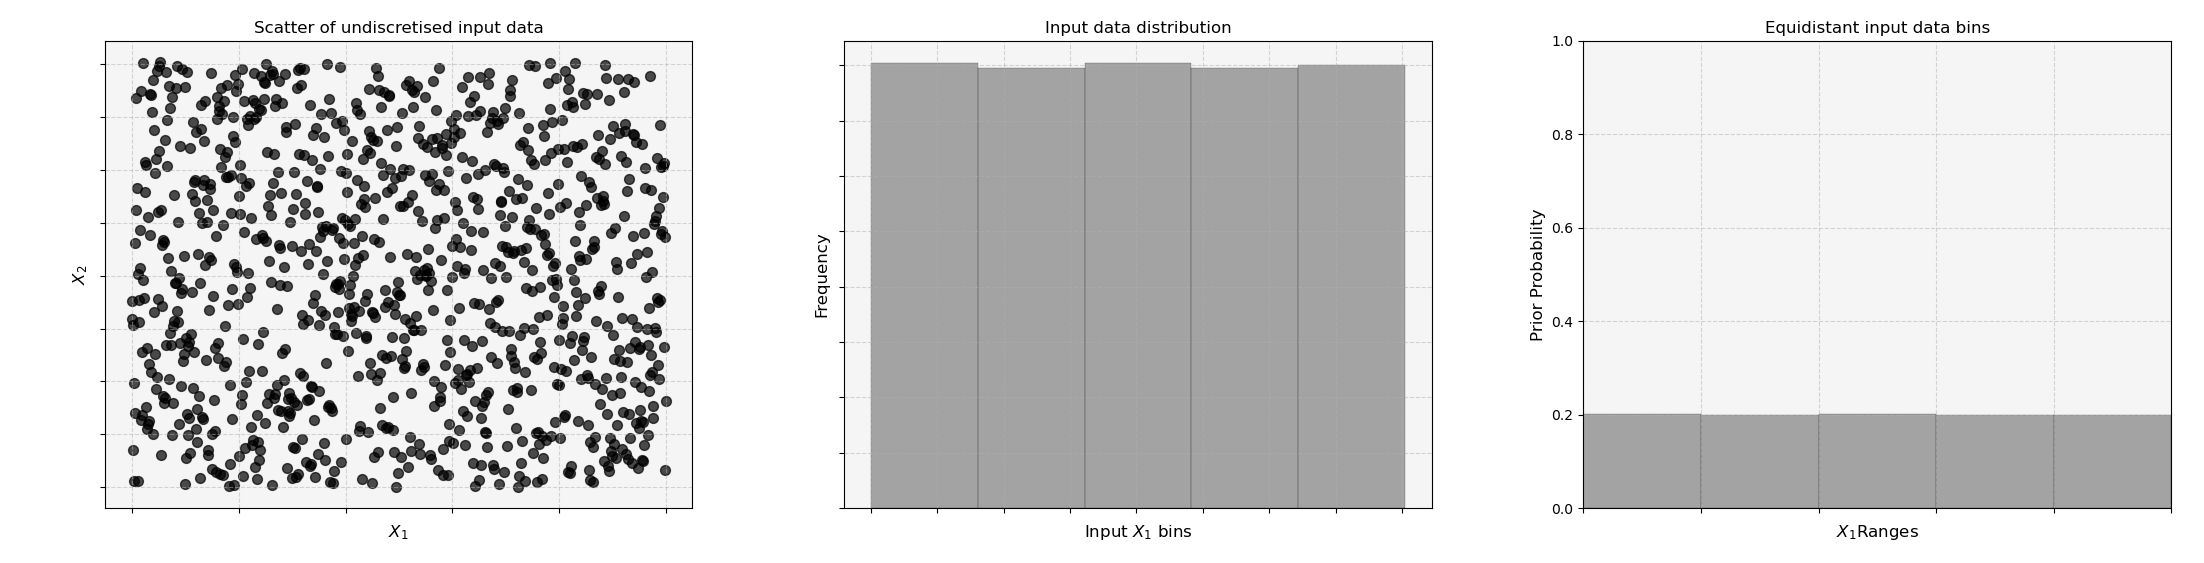
\includegraphics[width=0.8\textwidth]{figures/methodology/input_discretisation.png}
            \caption{\small inputs}\label{fig:input_dist_eg}
        \end{subfigure}
    \end{minipage}
    \begin{minipage}{\textwidth}
        \begin{subfigure}{\textwidth}
            \centering
            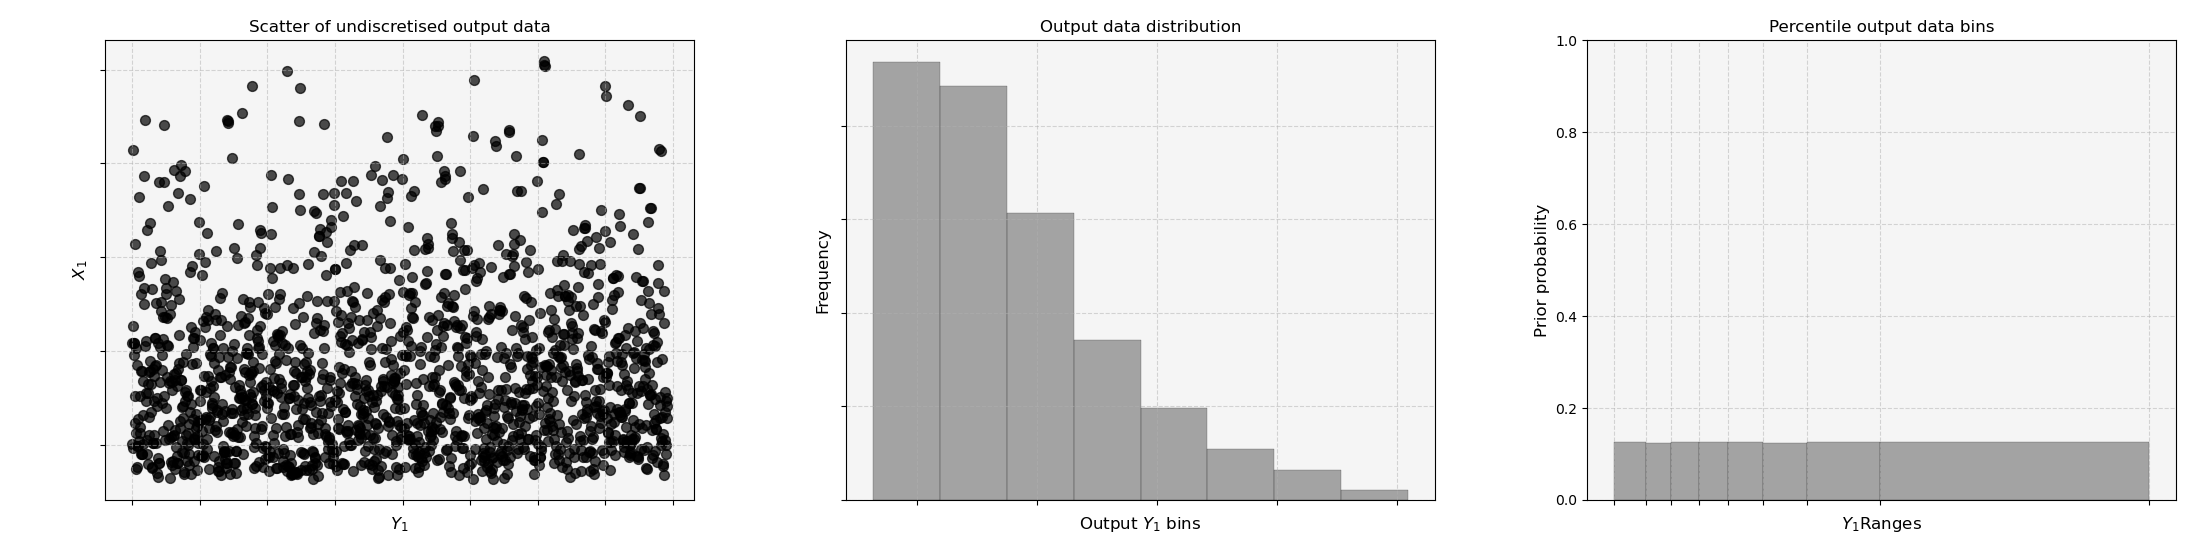
\includegraphics[width=0.8\textwidth]{figures/methodology/output_discretisation.png}
            \caption{\small outputs}\label{fig:output_dist_eg}
        \end{subfigure}
    \end{minipage}
    \caption{\small An example of the input distribution of a variable demonstrating the need for equidistant binning. An example of the output distribution of a variable demonstrating the need for percentile binning.}\label{fig:dists_eg}
\end{figure*}


The BN is configured at this stage to mirror the deterministic model, using the inputs selected in Step~\ref{sec:parameters} and the data collected in Step~\ref{sec:data}. The data is discretised either by equidistant binning or by percentiles, for inputs and outputs respectively.

BNs are designed to handle discrete distributions, which means that datasets need to be discretised into bins before they can be used. This discretisation process is necessary to convert continuous data into discrete categories or intervals that the BN can handle effectively. By discretising the dataset into appropriate bins, the BN can leverage the discrete nature of the variables and make probabilistic inferences. Discretisation is a method used in machine learning to transform continuous variables into discrete categories or bins.

For example, in~\cite{Griffiths2024}, two distinct methods of discretisation were employed: \textit{equal distance} and \textit{percentile binning}. For the inputs, the \textit{equal distance} approach was applied, while the \textit{percentile binning} method is implemented for the target. This differentiation allows for an effective and tailored discretisation process that accommodates the specific characteristics and requirements of the inputs and outputs.

Equal distance binning divides the range of a variable into a fixed number of equal-sized intervals or bins\@. This method assigns values to bins based on their proximity to the bin boundaries. Equal distance binning is commonly used for discretising input features in machine learning because it preserves the linear relationship between the variable values and allows for easy interpretation of the results. It can be particularly useful when the variable exhibits a linear trend or when the absolute values of the variable are important for the prediction task, making it the most appropriate method during the initial construction of the BN.\@ Referring to Figure~\ref{fig:input_dist_eg}, the input distribution of a variable demonstrates the need for equidistant binning.

On the other hand, percentile binning divides the data based on the distribution of the variable values. Each bin contains an equal number or percentage of data points, ensuring that the bins capture an approximately equal amount of information. Percentile binning is often preferred for discretising target or output variables in ML.\@ This is because output data distributions are typically less uniform. It can thus help handle class imbalance issues, i.e., bias, and create more balanced categories for classification tasks. By grouping data points based on their relative positions in the distribution, percentile binning can ensure that each bin represents a similar portion of the target variable, reducing the impact of outliers and enhancing model performance. Referring to Figure~\ref{fig:output_dist_eg}, the input distribution of a variable demonstrates the need for equidistant binning.  Overall, the selection of the appropriate discretisation method should be based on an understanding of the data distribution, the specific machine learning task, and the goals of the analysis. 

Once discretised into probability distributions, both inputs and outputs from training data configure the BN.~Here the BN learns the parameters and develops the causal relationships between them, i.e., populates the conditional probability tables with the prior distributions of the variables. In this context, the pre-configured and validated BN can then be employed to perform bi-directional inference in Step~\ref{sec:meth_decision}.

\subsection{\textbf{Step 6}: Model Validation and Testing}\label{sec:meth_validation} 

\begin{figure*}
    \centering
    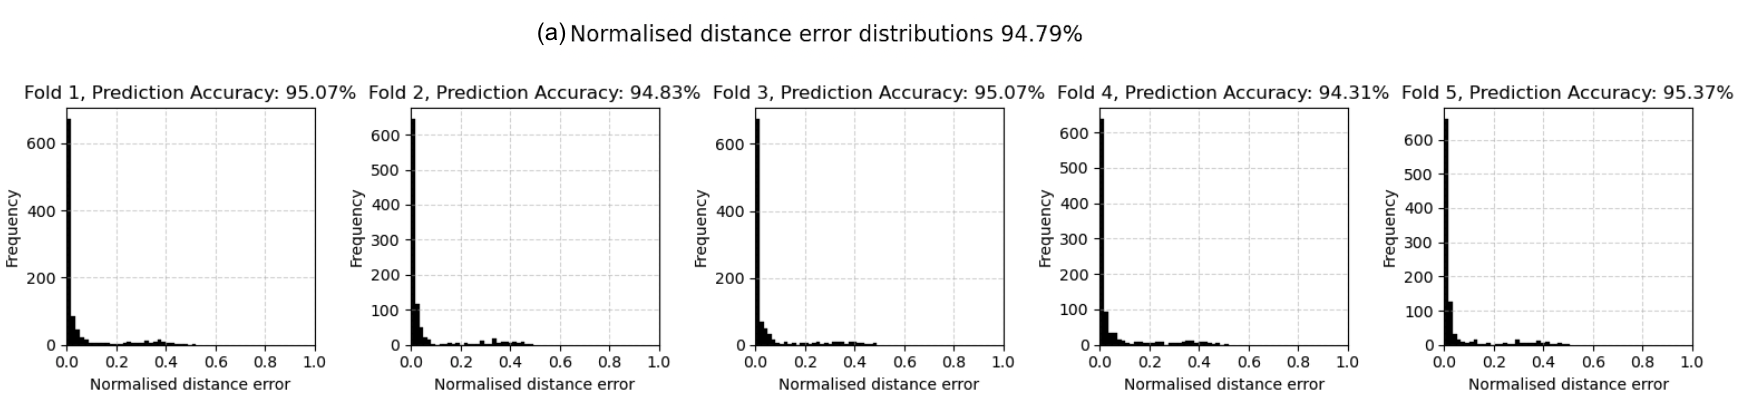
\includegraphics[width=\textwidth]{figures/validation_plots/PROCESS/st20_d1_7bins_folds.png}
    \caption{\small Normalised probability histograms with prediction accuracy values for the first 5 folds is shown for $d_{1}$ bin resolution = 7, dataset size = 10240.}~\label{fig:k-foldhistograms}
\end{figure*}

Validation is the term used to measure model accuracy. As part of the validation procedure and in order to avoid bias, a partitioning technique was used to partition the dataset into training and testing in $k$ distinct manners, known as $k$-fold cross-validation. This means the BN was built, and then validated $k$ times, with $k$ unique combinations of training and $k$ testing sets. The ratio of the split between training and testing sets in each fold is determined by the number of folds used to split the dataset by $1/k$, e.g., 3 folds will have a test split size of $1/3 = 33\%$. 

In order to quantify how well the model makes predictions compared to the analytical response, the predicted values were compared with the actual values in the testing data. In traditional machine learning evaluation methods like Root Mean Square Error (RMSE), the predictions and actual values are typically scalar values, such as numerical measurements or continuous variables. However, in the context of BNs, the outputs are probabilistic, distributions, or categorical variables rather than single numerical values. As a result, standard evaluation metrics like RMSE are not directly applicable, and alternative or custom approaches must be used to assess the performance of BN models. This can done either by calculating the difference between the mean of the predicted bin and the simulated value in the testing data, or by calculating the difference between the mean of the predicted bin and the mean of the bin in which the actual simulated value lies.

The NDE is a measure used to assess the relative magnitude of the distance error in relation to the range of values in a given bin. It helps to put the distance error into perspective and make it comparable across different bin ranges. By dividing the distance error by the difference between the maximum and minimum bin range values, a normalised distance error is obtained that takes into account the scale and range of the data. This normalisation allows for a fair comparison of the distance error across different bin ranges, providing a standardised measure of the error~\cite{Conti2019}.

\subsubsection{Validation of the proof-of-concept surrogate}\label{sec:res_validation}

\begin{figure}[h]
    \centering
    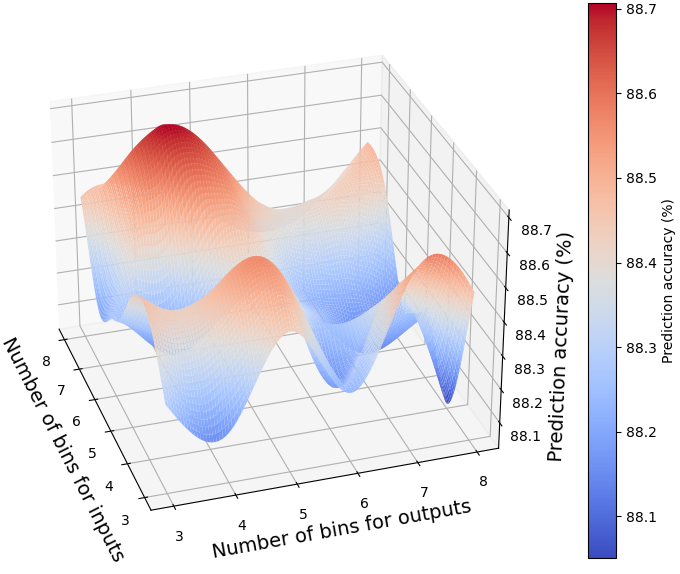
\includegraphics[width=0.9\columnwidth]{figures/validation_plots/PROCESS/SA_3D_trimmed_39.png}
    \caption{\small A 3D surface plot displaying the average accuracy of predictions for $d_{1}$ errors while investigating variations in bin resolution.}~\label{fig:3D_SA_trimmed_39_D1}
\end{figure}

This section details the implementation of Step~\ref{sec:meth_validation} using the dataset from the proof-of-concept study~\cite{Griffiths2024}. Specifically, this section provides an overview of the outcomes obtained through $k$-fold cross-validation, and presents the findings from hyperparameter tuning. The validation process was conducted to assess the BN's predictive accuracy and reliability, and to identify the optimal hyperparameters for configuring the model. The results of the validation process provide valuable insights into the performance of the BN model and inform the selection of hyperparameters for future model development.

Using the data, calibration of hyper-parameters (such as bin resolution and dataset sizes) were examined by exploring two factors: (i) utilising three distinct dataset sizes and, (ii) experimenting with different bin resolutions during discretisation. The objective was to determine how modifying these paramters impacted the BN's ability to make predictions that could be usefully interpretted by the user. Consequently, for (i) this meant dataset sizes of 1400, 5120, and 10240 and, for (ii), incrementally increasing the number of bins used in discretisation between inputs and outputs for all combinations between 3 and 12, respectively. For (i), it was found that configuring the BN using the largest dataset resulted in the highest prediction accuracy. For (ii) the findings are presented in~\ref{fig:3D_SA_trimmed_39_D1}, illustrating that the model exhibited optimal performance when and input data was discretised into 7 bins and output data into 5 bins, respectively. In general, the average prediction accuracy for $d_{2}$ errors tends to be higher than that for $d_{1}$ errors, except in the case of using high bin resolutions.

To enable $k$-fold cross-validation, the dataset was split into 10 folds. 10 fold cross-validation aligns with the recommendation by Marcot et al.~\cite{Marcot2021}, who support the prevalent use of $k$=10 for BNs in literature. Plotting the NDE in a histogram provides a good illustration of model performance, see Figure~\ref{fig:k-foldhistograms}. The resulting validation plot distributions in~\ref{fig:k-foldhistograms} offers a clear representation of the model's predictive capabilities. Overall, when observing the distribution of the d1 plots for all 10 folds, it can be noted that the BNM built on 10,000 data points, seems to predict the correct response with an average $\sim$95\% accuracy.

This high level of accuracy underscores the model's robustness and reliability in making predictions. It also highlights the value of using a substantial dataset for building the model, as in~\cite{Griffiths2024}. These findings contribute to the growing body of evidence supporting the use of BNs in making accurate predictions, and they underscore the importance of careful model construction and validation.

The results from the hyper-parameter calibration provide valuable insights into the performance of the BN model. Two key factors were examined: dataset size and bin resolution during discretisation. The investigation found that the size of the dataset used to configure the BN significantly impacts its predictive accuracy. Specifically, the largest dataset (10,240) yielded the highest prediction accuracy. This suggests that the BN model benefits from a larger volume of data, likely because it provides a more comprehensive representation of the underlying distributions and dependencies. Whilst this is not a groundbreaking realisation, it is a useful reminder that the quality of the data used to configure the BN is crucial to its performance. The findings also highlight the importance of collecting a sufficient amount of data to ensure the model's accuracy and reliability, and ensures that these models are not overfitting to the training data. Going forward, this study will inform the collection of data for future BN models, ensuring that the dataset is sufficiently large to support accurate and reliable predictions, especially when the model is used to make critical decisions in engineering design with fusion developers.

The bin resolution during discretisation also played a crucial role in the model's performance. The optimal performance was observed when the input data was discretised into 7 bins and the output data into 5 bins. This indicates a balance is needed in the bin resolution. Too few bins may oversimplify the data, losing important information, while too many bins can lead to overfitting, where the model becomes too tailored to the training data and performs poorly on new data.

\begin{figure*}[t]
    \centering
    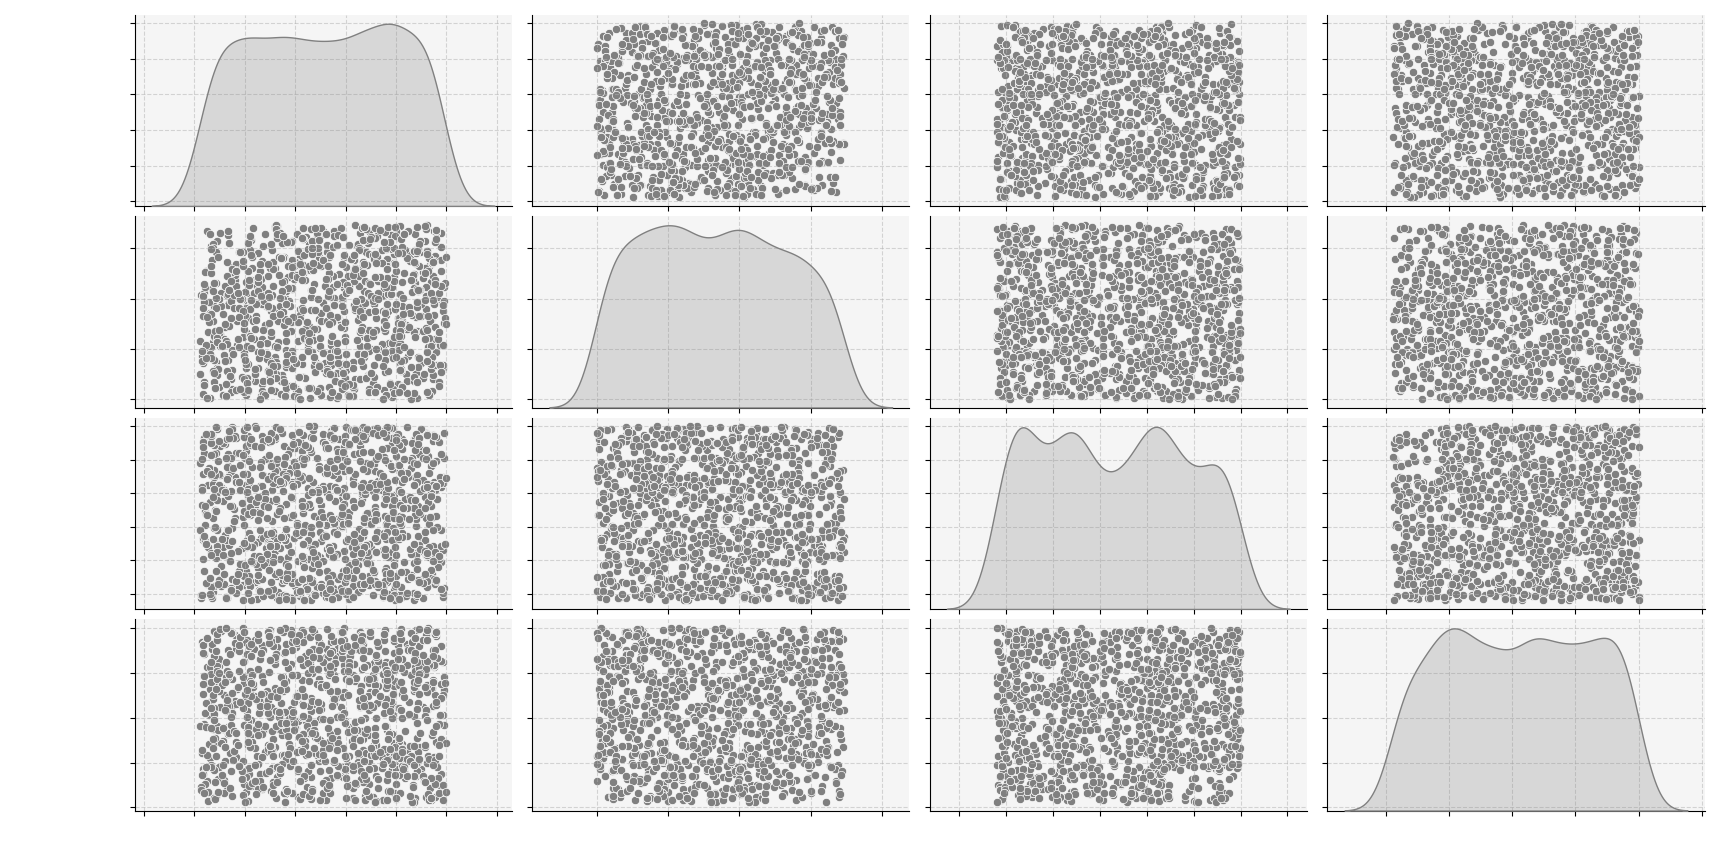
\includegraphics[width=0.8\textwidth]{figures/TE_results/4grid_scatter.png}
    \caption{\small A 4$\times$4 scatter-grid to illustrate the sampling of an example input space. The scatter-grid is a visual representation where each point represents a unique combination of input values. The scatter-grid is a useful tool for visualising the distribution of the input space and identifying any gaps or biases in the data.}\label{fig:scatter_sampling}
\end{figure*}

Interestingly, the average prediction accuracy for $d_{2}$ errors was generally higher than that for $d_{1}$ errors, except when using high bin resolutions. This is largely down to how the model handles the different types of errors. The $d_{1}$ error measures the difference between the mean of the predicted bin and the simulated value in the testing data, while the $d_{2}$ error measures the difference between the mean of the predicted bin and the mean of the bin in which the actual simulated value lies. Thus, the likelihood that the correct bin is predicted is higher for $d_{2}$ errors, as it is based on the mean of the bin rather than the actual value. This is an important consideration when interpreting the results and understanding the model's performance. The results suggest that the model may be more sensitive to the bin resolution for $d_{1}$ errors, and care should be taken when choosing the bin resolution in this case.

These findings contribute to a deeper understanding of how hyper-parameter choices affect the performance of BN models, and can guide the selection of these parameters in future work by providing a clear indication of the optimal dataset size and bin resolution to benchmark the model. This will help to ensure that the BN model is configured to provide accurate and reliable predictions, and that the results can be interpreted with confidence.

\subsection{\textbf{Step 7}: Design Constraint Decision Support}\label{sec:meth_decision}

In this step application of the BN to provide decision support for engineering design is impleented through Bayesian bi-directional inference. Forward inference involves updating prior assumptions of inputs, utilising available evidence to give the output response. Conversely, reverse inference involves estimating the inputs given the output. The ability to perform reverse inference stems from the fact that once a BN has learned the parameters, it no longer differentiates between inputs and outputs. This characteristic allows the network to infer in both directions, making it possible to predict inputs based on output data., such as determining input ranges for optimal performance based on a desired output using reverse inference. This demonstrates an update from previous work with greater depth and analysis given. 

\section{Case Study Appplication}\label{sec:res_decision} 

In this section, the BN model is applied to a case study using the methodological framework outline in~\ref{sec:methodology} to demonstrate its utility in providing decision support for engineering design. The case study focuses on the application of the BN to determine input ranges for optimal performance based on a specified output. This application is particularly relevant in the context of fusion reactor design, where engineers and researchers need to identify the input parameters that will yield the desired output performance. Section~\ref{sec:res_reverse} delves into the outcomes of reverse inference with the BN, emphasising the prediction of ranges for economic fusion parameters from uncertain data. Results can provide decision support for components, such as determining input ranges for optimal performance based on a desired output using reverse inference. This demonstrates an update from the proof-of-concept with greater depth and analysis given in Step 7 (\ref{sec:meth_decision}).

For \textbf{Step 1}: Define Design Variables (\ref{sec:design}), the aim was to model a whole reactor system, determining how important output parameters vary with certain inputs by studying their sensitivity to one another. For \textbf{Step 2}: (~\ref{sec:deterministic}), the deterministic  model used was `PyTOK', a systems code that finds optimum working point using a series of 0D and 1D approximations that model all subsystems. For \textbf{Step 3}: (\ref{sec:parameters}), the important parameters for the surrogate model were carefully selected based on insights from the PyTOK model, a comprehensive tool for fusion reactor analysis. The chosen input parameters include: 

\textbf{Major Radius ($R$)}: This parameter represents the distance from the center of the torus to the center of the plasma. In fusion terminology, it defines the size of the plasma confinement region and influences key plasma stability characteristics. A larger major radius typically allows for increased plasma volume, enhancing overall fusion performance.

~\textbf{Aspect Ratio ($A$)}: The aspect ratio signifies the ratio of the major radius ($R$) to the minor radius ($a$), which is the radius of the cross-sectional circle of the torus. Higher aspect ratios are characteristic of spherical tokamaks, a specific type of fusion device. Aspect ratio plays a crucial role in shaping the plasma equilibrium and can affect plasma stability and confinement properties.

~\textbf{Effective Ion Charge ($Z_{\text{eff}}$)}: This parameter serves as a measure of the average charge state of ions within the plasma. It is calculated by summing the square of the charge of each ion species, weighted by their respective densities. A higher effective ion charge may indicate the presence of impurities in the plasma, which can lead to increased energy losses and impact fusion performance.

~\textbf{Toroidal Field on Plasma ($B_{\text{T}}$)}: The toroidal field refers to the magnetic field that wraps around the torus in the direction of the major radius ($R$). It plays a crucial role in confining the plasma along the toroidal direction and is typically much stronger than the poloidal field, which confines the plasma in the radial direction. The strength of the toroidal field influences plasma stability, confinement, and overall fusion performance. 

The chosen output parameters were:

~\textbf{Engineering Gain ($Q_{\text{eng}}$)}: This factor is defined as the ratio of the power produced by the fusion reactions to the external heating power. Thus, a $Q_{\text{eng}}$=1 represents breakeven, where the power generated from fusion reactions in a plasma exceeds that of the external power needed to create the plasma state. Achieving a high $Q_{\text{eng}}$ is indicative of the reactor's ability to sustain fusion reactions efficiently.

~\textbf{High Grade Waste Heat ($H$) (MWt)}: $H$ refers to the thermal energy harnessed in a thermodynamic cooling cycle by the breeder blanket for efficient conversion into usable heat or electricity. The heat can also be utilised for various industrial processes, district heating, or power generation, maximising the reactor's energy output and overall efficiency~\cite{Griffiths2022}. Efficient utilisation of waste heat maximizes the overall efficiency of the fusion reactor if non-electric applications can be implemented alongside electricity generation~\cite{Hidalgo-Salaverri2023}.

~\textbf{Net Electrical Output ($E$) (MWe)}: This parameter quantifies the amount of electrical power generated by the fusion reactor. Achieving a high $E$ signifies the effectiveness of the fusion reaction in producing usable electrical energy. Thus, an elevated $E$ can contribute significantly to the grid, meeting energy demands to provide baseload power and ultimately reducing reliance on fossil fuels or other non-renewable sources.

~\textbf{Capital Cost ($C$) (million USD)}: This represents the overnight cost of building the fusion reactor. It is a crucial factor in assessing the economic feasibility and viability of implementing fusion energy technology. 

For \textbf{Step 4}: (\ref{sec:data}), the input space between the parameter limits was sampled using the identical Sobol methods to that in\cite{Griffiths2024}. Data was collected from the PyTOK model to produce a dataset size of 10,000. See Figure~\ref{fig:scatter_sampling}. For \textbf{Step 5}:,~\ref{sec:BNconfiguration}, the BN was configured to replicate PyTOK using the inputs outlined in above for~\ref{sec:parameters}, see Figure~\ref{fig:BN2}. The data was discretised using the optimal bin resolution of 7 for the inputs and 5 for the outputs, as determined in the hyper-parameter calibration. The BN was then validated using 10(k)-fold cross-validation to assess its predictive accuracy and reliability. The validation process provided valuable insights into the performance of the BN model and informed the selection of hyperparameters for future model development. See the Appendix~\ref{appendix:prediction_accuracy} figure~\ref{fig:k-foldhistogramsTE}.

\begin{figure}[t]
    \centering
    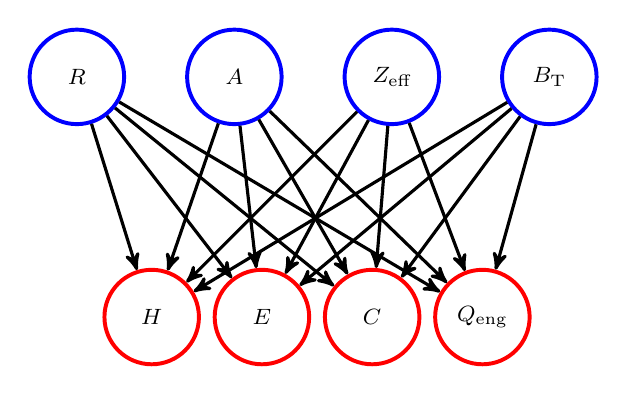
\begin{tikzpicture}[node distance=1.5cm, font=\footnotesize, align=center, >=stealth', line width=0.5mm]
        % Define colors
        \definecolor{lightgreen}{rgb}{0.56, 0.93, 0.56}
        \definecolor{lightred}{rgb}{0.98, 0.5, 0.45}

        % Nodes
        \node[draw, circle, draw=blue, text=black, minimum size=1.2cm] (input1) {$R$};
        \node[draw, circle, draw=blue, text=black, right of=input1, xshift=0.5cm, minimum size=1.2cm] (input2) {$A$};
        \node[draw, circle, draw=blue, text=black, right of=input2, xshift=0.5cm, minimum size=1.2cm] (input3) {$Z_{\text{eff}}$};
        \node[draw, circle, draw=blue, text=black, right of=input3, xshift=0.5cm, minimum size=1.2cm] (input4) {$B_{\text{T}}$};

        \node[draw, circle, draw=red, text=black, below=1.8cm of input2, xshift=-1.05cm, minimum size=1.2cm] (output1) {$H$};
        \node[draw, circle, draw=red, text=black, below=1.8cm of input2, xshift=0.35cm, minimum size=1.2cm] (output2) {$E$};
        \node[draw, circle, draw=red, text=black, below=1.8cm of input2, xshift=1.75cm, minimum size=1.2cm] (output3) {$C$};
        \node[draw, circle, draw=red, text=black, below=1.8cm of input2, xshift=3.15cm, minimum size=1.2cm] (output4) {$Q_{\text{eng}}$};

        % Edges
        \foreach \i in {1,...,4} {
            \foreach \j in {1,...,4} {
                \draw[->, line width=0.4mm] (input\i) -- (output\j);  % Decreased line width
            }
        }
    \end{tikzpicture}
    \caption{\small Graphical representation of Bayesian Network where nodes represent the input variables (Major Radius $R$, Aspect Ratio $A$, Effective Ion Charge $Z_{\text{eff}}$, Toroidal Field on Plasma $B_{\text{T}}$) and the output variables (High Grade Wasteheat $H$, Net Electrical Output $E$, Capital Cost $C$, and Engineering Quality $Q_{\text{eng}}$) to the analytical model.}\label{fig:BN2} 
    \vspace{-15pt}
\end{figure}

%%\subsection{Forward Inference}\label{sec:res_forward}
\subsection{\textbf{Bayesian Reverse Inference}}\label{sec:res_reverse}

Corresponding to \textbf{Step 7} in~\ref{sec:methodology}, this section presents the outcomes of reverse inference, employed to predict the input parameters that are most likely to yield a specified output, such as minimising $C$. In this context, modelling a reactor with elevated $E$, $H$, and $Q_{\text{eng}}$ within specific ranges is indicative of aiming for a high-performance reactor system. 

$C$, was increased between each result, ranging from \$3.4--3.8 billion to \$4.4--6.5 billion. The aim of this approach was to illustrate the variation in the posterior distributions of the input parameters contingent on $C$. The outcomes of the reverse inference are depicted in Figures~\ref{fig:BN_case_study} and~\ref{fig:BN_case_study2}, which illustrate the posterior distributions of the fusion input parameters (highlighted in red) for the selected output parameter bins (in green). The findings suggest that for a reactor with a $C$ of \$3.4--3.8 billion, and output parameters $E$ of 100--180 MWe, $H$ of 800--1100 MWt, and $Q_{\text{eng}}$ of 1.70--2.00, the most probable input parameters are a $R$ of 3.02--3.27 m, an $Z_{\text{eff}}$ of 1.85.2.50 and a $B_{\text{T}}$ of 4.06--5.03T. The posterior distribution of $A$ is flatter than the other input parameters.  

In contrast, for a reactor with a $C$ of \$4.2--4.8 billion, and output parameters $E$ of 80--150 MWe, $H$ of 650--850MWt, and $Q_{\text{eng}}$ of 1.70, the most probable input parameters are a $R$ of 3.76--4.00 m, an $A$ of 1.80--1.97, and a $B_{\text{T}}$ of 5.51--6.00T. The posterior distributions of $Z_{\text{eff}}$ is flatter than the other input parameters, with the largest posterior occuring between 1.20--1.52.

\begin{figure*}[t]
    \centering
    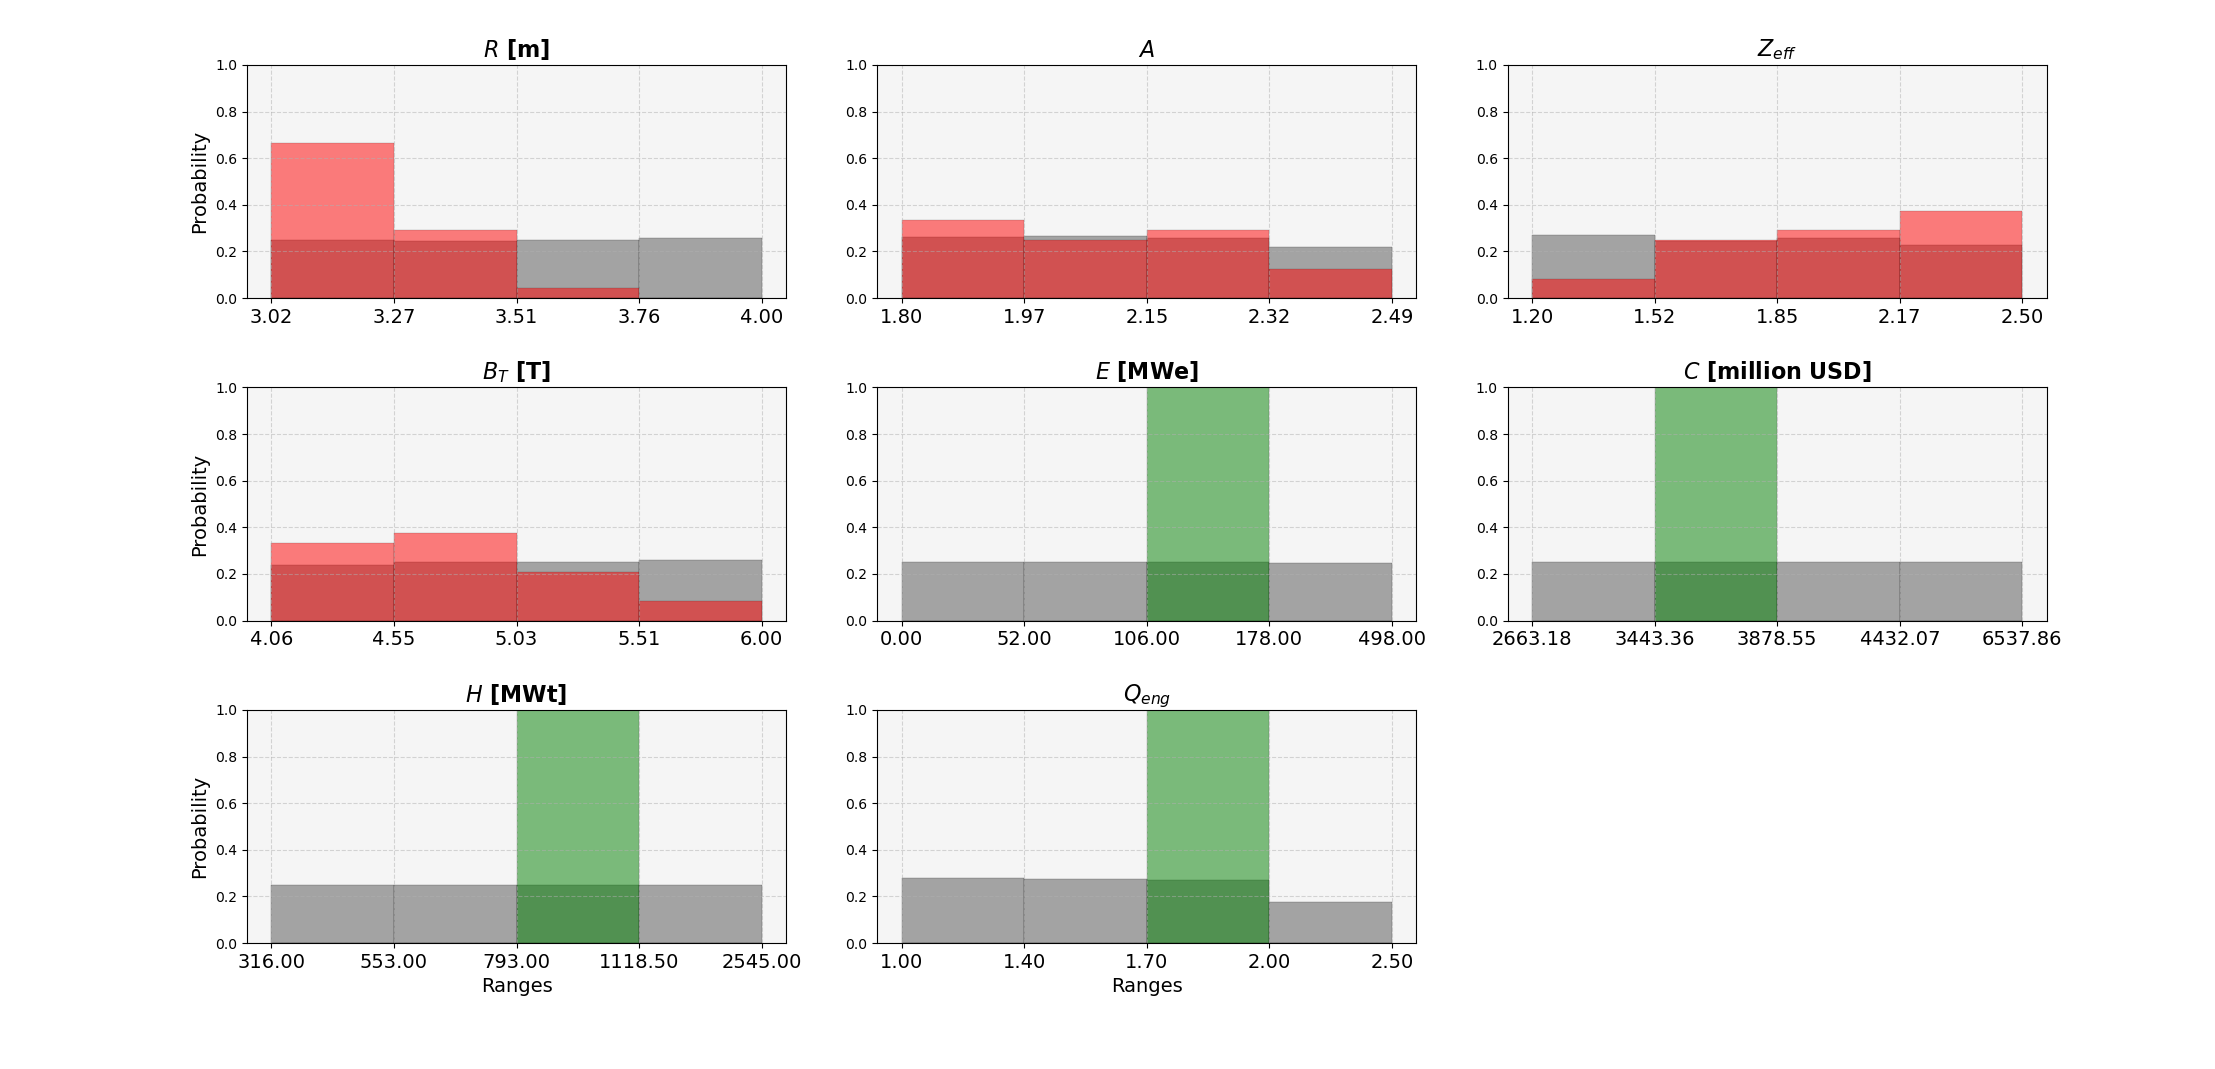
\includegraphics[width=0.9\textwidth]{figures/TE_results/config(44)_4outputs/Figure_4_v2.png}
    \caption{Resulting posterior distributions depicted in red (variables: Major Radius $R$, Aspect Ratio $A$, Effective Ion Charge $Z_{\text{eff}}$, Toroidal Field on Plasma $B_{\text{T}}$) for reverse
    inference on the selected green bins (High Grade Wasteheat $H$, Net Electrical Output $E$, Capital Cost $C$, and Engineering Quality $Q_{\text{eng}}$) after updating the marginal prior beliefs (grey).}\label{fig:BN_case_study}
\end{figure*}

\begin{figure*}[t]
    \centering
    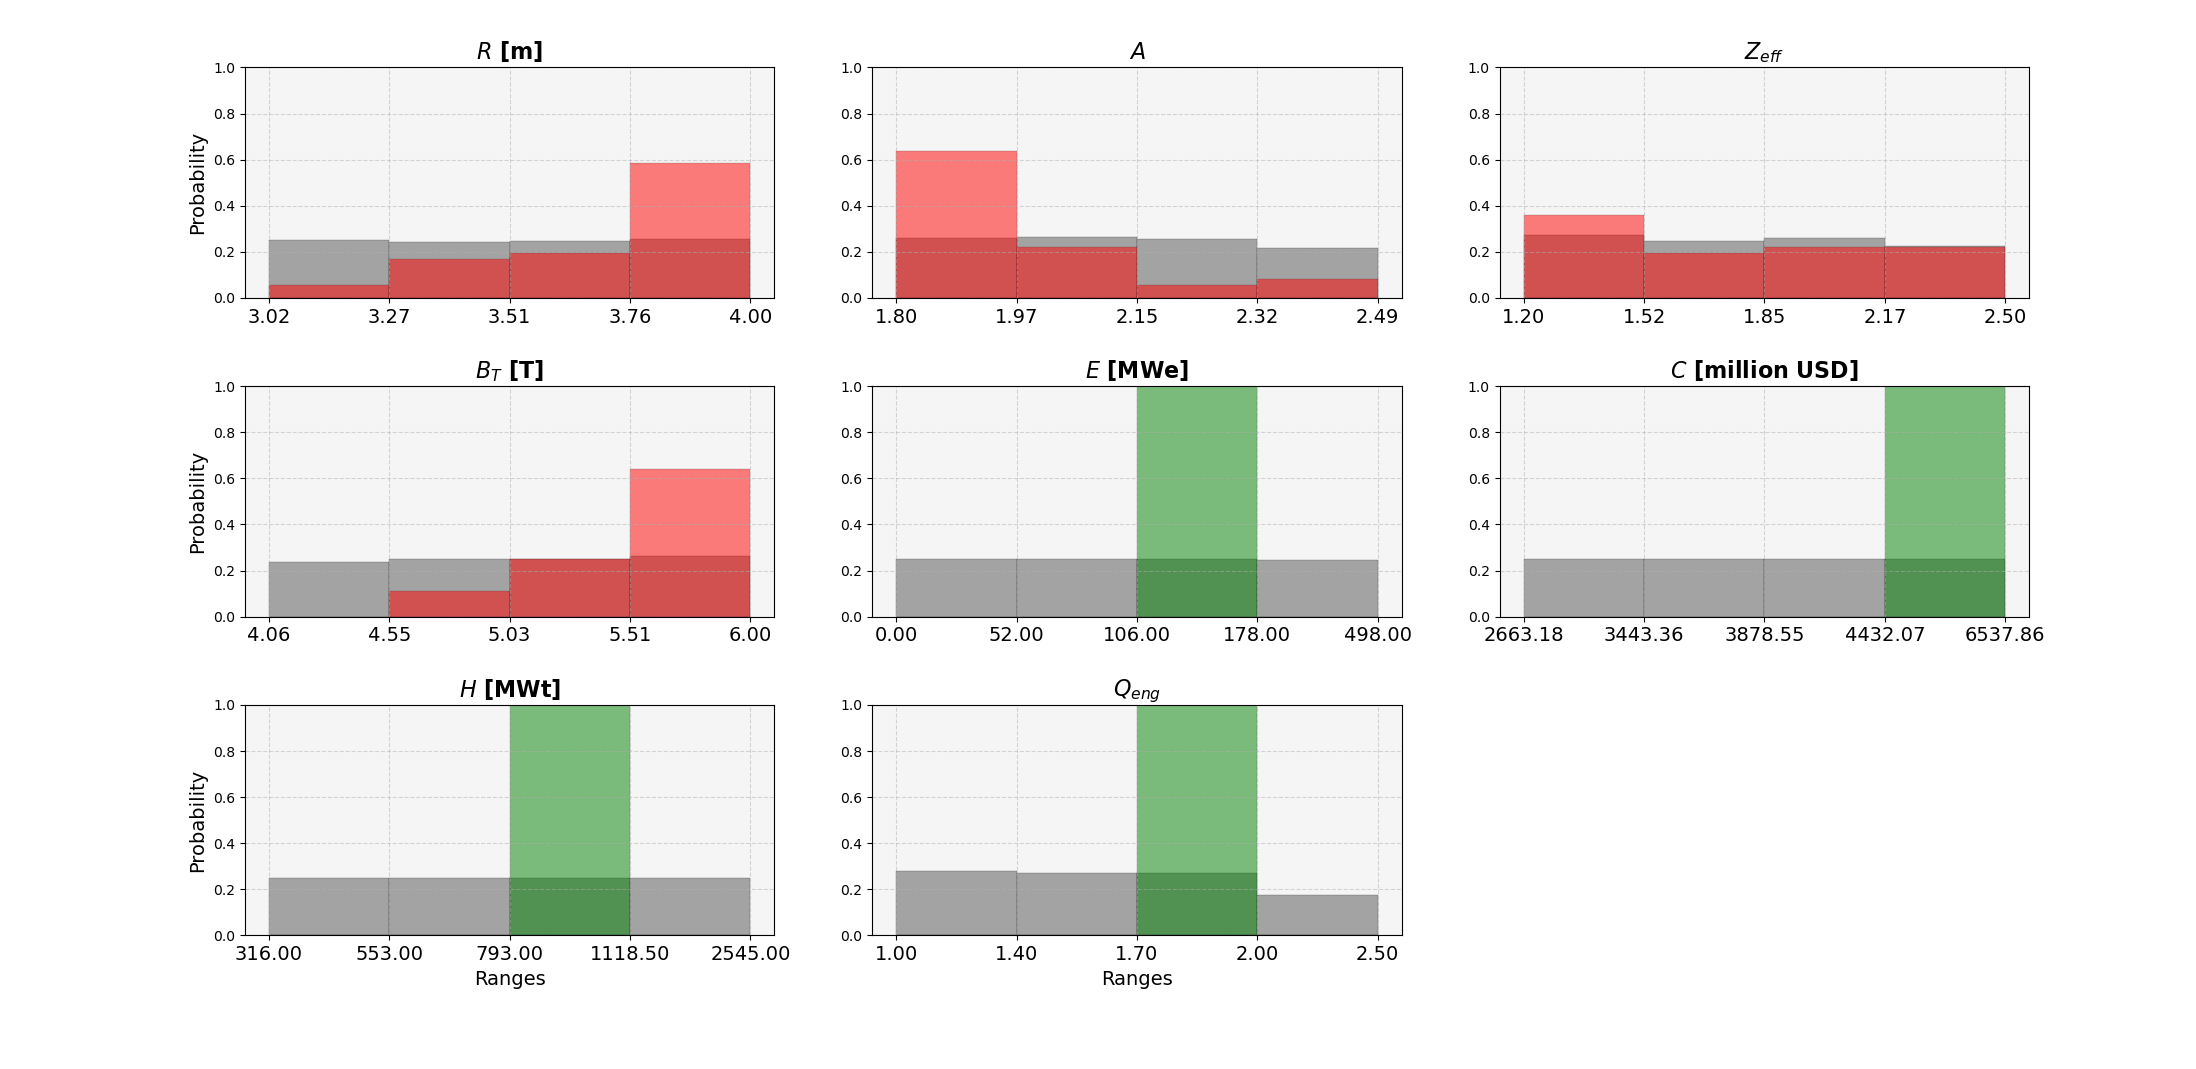
\includegraphics[width=0.9\textwidth]{figures/TE_results/config(44)_4outputs/Figure_5_V2.png}
    \caption{Resulting posterior distributions depicted in red (variables: Major Radius $R$, Aspect Ratio $A$, Effective Ion Charge $Z_{\text{eff}}$, Toroidal Field on Plasma $B_{\text{T}}$) for reverse
    inference on the selected green bins (High Grade Wasteheat $H$, Net Electrical Output $E$, Capital Cost $C$, and Engineering Quality $Q_{\text{eng}}$) after updating the marginal prior beliefs (grey).}\label{fig:BN_case_study2}
\end{figure*}

\section{Discussion}\label{sec:Discussion}

%%\subsection{Forward Inference}\label{sec:disc_forward}

\subsection{Reverse Inference}\label{sec:disc_reverse}

The outcomes of the reverse inference analysis provide fusion developers with valuable insights into optimising the design parameters of fusion reactors and their components. The ability to identify the most probable input parameters for a given set of output parameters, can significantly inform the design process. By examining the posterior distributions of fusion input parameters in relation to specified output parameters, such as elevated values of energy output ($E$), fusion power ($H$), and $Q_{\text{eng}}$, developers can identify the most probable input parameter ranges that lead to high-performance reactor systems. The results highlight the ability to use the model across different stages of the design process, and it is expected to provide valuable insights for the development of future fusion power plants. In addition, the ambiguity of the model and its ability to handle data from any input-output model highlight the flexibility and adaptability of the BN, making it a valuable tool for fusion developers.

The analysis reveals a significant shift in the most probable input parameters for fusion reactor design, contingent upon the reactor's $C$. For reactors with a lower $C$ (\$3.2-3.8 billion), optimal parameters tend towards a smaller $R$, higher $Z_{\text{eff}}$, and lower $B_{\text{T}}$, aligning with specified output parameter ranges. The posteriors of $A$ illustrates a broader distribution compared to other input parameters. This suggests that for lower $C$ machines, there is increased flexibility in selecting the desired value for $A$. However, as $C$ is increased (\$4.4-6.5 billion), the most probable parameters shift, indicating a need for a larger $R$, reduced $A$, reduced $s_{\text{eff}}$, and increased $B_{\text{T}}$ to meet the specified output parameters.

The observed decrease in $A$ with increased $C$ can be interpreted through the lens of engineering trade-offs. As $C$ rises, design considerations may prioritise aspects like scalability and efficiency over compactness. A larger $R$ accommodates more plasma volume, potentially enhancing overall reactor performance and output, albeit at the expense of increased material and construction costs. Moreover, a lower $A$ may be favored in larger-scale reactors to optimise plasma stability and confinement, aligning with the operational demands of a higher-budget project. 

This model-based insight underscores the intricate interplay between reactor design parameters and capital investment. The shift in optimal parameters with varying $C$s highlights the nuanced considerations that developers must navigate to achieve cost-effective and high-performance fusion reactor designs. By interpreting these results, developers can strategically tailor design choices for reactor components, such as toroidal magnets and vacuum vessels, to optimise performance within budgetary constraints, fostering advancements in fusion energy technology.

These insights enable developers to make informed decisions during the design optimisation process. By focusing on the input parameter ranges associated with desired output parameters, developers can refine their reactor designs to enhance performance while considering cost constraints. Additionally, this information can guide the selection of input parameters to achieve specific performance targets, such as maximising energy output or $Q_{\text{eng}}$, within budgetary limitations. However, it is important to note that these results are based on the current state of knowledge and technology. As such, it would be beneficial to continually update the Bayesian model as new data becomes available. This could include results from experimental reactors, advancements in plasma physics, or changes in manufacturing costs.

\section{Conclusion and Further Work}\label{sec:conc}

In summary, probabilistic Bayesian inference serves as a powerful tool for enhancing fusion research by providing a comprehensive framework for integrating data, quantifying uncertainties, optimising experimental design, supporting decision-making, and managing risks. By leveraging Bayesian methods in conjunction with existing approaches, fusion researchers can gain deeper insights into reactor behaviour, accelerate the pace of innovation, and advance the development of practical fusion energy solutions.

\section{Acknowledgments}
This research was supported by the EPSRC (Engineering and Physical Sciences Research Council, UK) Nuclear Energy Futures Centre for Doctoral. Training in Nuclear Energy (NEF CDT). Other research studies under the NEF CDT involving Thomas Griffiths are supported in part by Tokamak Energy Ltd, UK. Views and opinions expressed are however those of the author(s) only a do not nsolidloosely dottedecessarily reflect those of Tokamak Energy Ltd.


\bibliographystyle{IEEEtranN}
\bibliography{library}

\begin{appendices}
    \section{Appendix: Prediction Accuracy}\label{appendix:prediction_accuracy}

\begin{table}[h]
    \centering
    \resizebox{\columnwidth}{!}                         \\ \cline{3-8} 
    \multicolumn{2}{|l}{}                                                           & \multicolumn{3}{c|}{$d_{1}$} & \multicolumn{3}{c|}{$d_{2}$}                   \\ \hline
    \multicolumn{2}{|c|}{Dataset size} &
        \multicolumn{1}{l|}{1400} &
        \multicolumn{1}{l|}{5120} &
        \multicolumn{1}{l|}{10240} &
        \multicolumn{1}{l|}{1400} &
        \multicolumn{1}{l|}{5120} &
        10240 \\ \hline
    \multicolumn{1}{|c|}{\multirow{3}{*}{Bin resolution}} & \multicolumn{1}{l|}{5}  & 92.73  & 92.84  & 93.13 & 96.36 & 96.76                     & 96.73 \\ \cline{2-2}
    \multicolumn{1}{|c|}{}                                & \multicolumn{1}{l|}{7}  & 93.74  & 94.08  & 94.79 & 96.98 & 96.79                     & 97.00 \\ \cline{2-2}
    \multicolumn{1}{|c|}{}                                & \multicolumn{1}{l|}{10} & 89.37  & 91.20  & 90.86 & 88.25 & \multicolumn{1}{r}{89.75} & 89.40 \\ \hline
    \end{tabular}%
    }
    \caption{\small A table displaying the average accuracy of predictions for $d_{1}$ and $d_{2}$ errors while investigating variations in both (i) the size of the dataset and (ii) the resolution of bins.}
    \label{tab:prediction_accuracy}
\end{table}

\begin{figure*}[h]
    \centering
    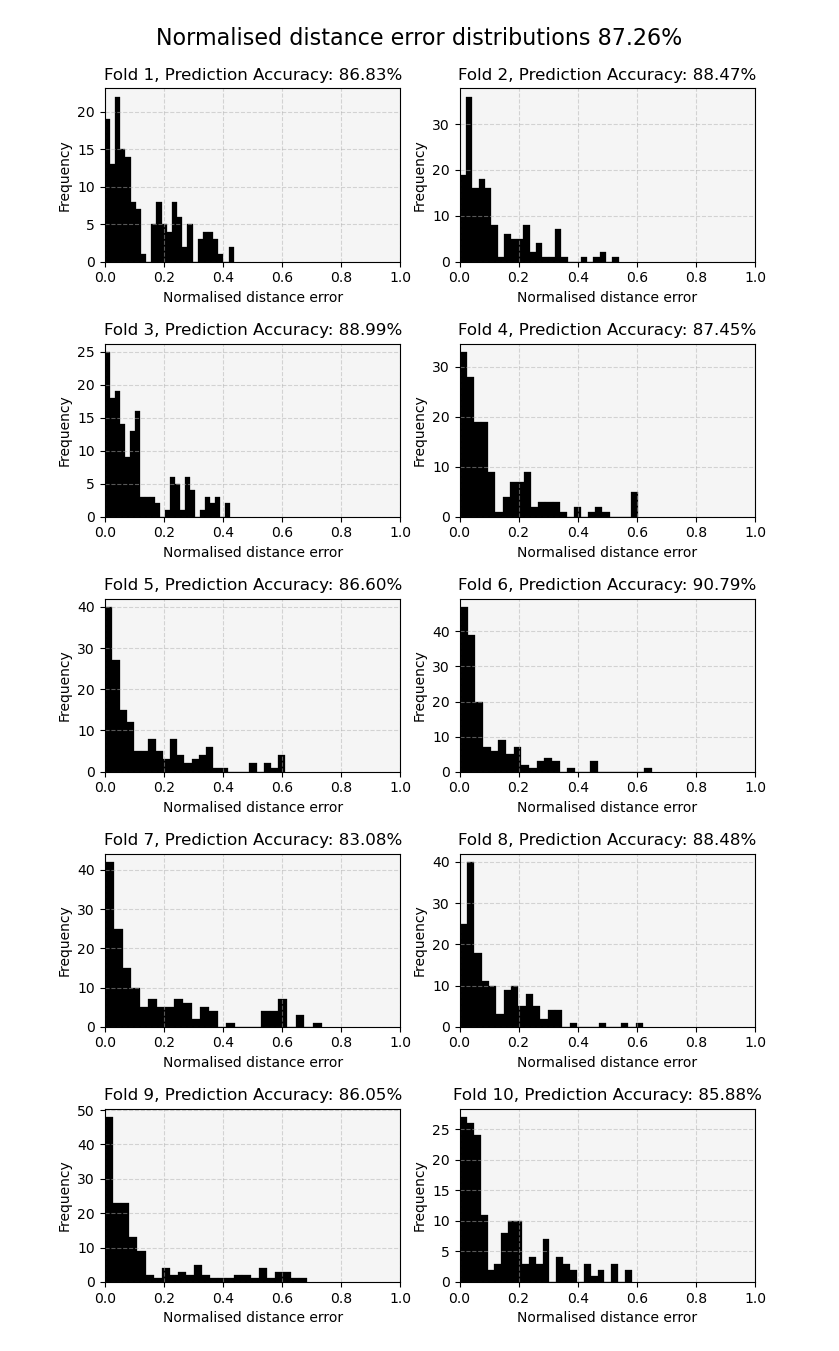
\includegraphics[width=0.65\textwidth]{figures/validation_plots/TE/k-fold_two_outputs.png}
    \caption{\small Normalised probability histograms with prediction accuracy values for each fold is shown for $d_{1}$ bin configuration: inputs (7) outputs (5), dataset size = 10240.}~\label{fig:k-foldhistogramsTE}
\end{figure*}
 \end{appendices}

\end{document}